\documentclass[final]{beamer}
\usetheme{Boadilla}
\usepackage{siunitx}
\usepackage{amsmath}
\usepackage{graphicx}
\usepackage[labelformat=empty]{caption}
\usepackage{verbatim}
\usepackage[orientation=portrait,size=a2]{beamerposter}
\usepackage[absolute,overlay]{textpos}
\setbeamertemplate{footline}[frame number]{}
\setbeamertemplate{navigation symbols}{}

\title{Optimising the design of buffer preparation in bioprocessing facilities}
\institute[UCD]{University College Dublin}
\date{\today}
\subtitle{MSc in Business Analytics (Part Time) 2015--2017}
\author{Sean Tully}



%==the poster content
\begin{document}
    \begin{frame}[t]
        \begin{columns}
            \column{0.1\textwidth}
                \begin{figure}
                    \centering
                    
\includegraphics[angle=0,scale=0.08]{ucd_logo.png}
                \end{figure}
            \column{0.85\textwidth}
            %\centering MSc in Business Analytics -- Dissertation\\
            \centering
            \vspace{0.2cm}
            
            \Huge{\textbf{Optimising the design of buffer preparation in
                 bioprocessing facilities}}
                 
            \huge \emph{Author: Sean Tully \quad \quad Supervisor: Prof.
                Michael O'Neill}
                
            \huge{M.Sc. Business Analytics -- 2017}
        \end{columns}
        
        \vspace{0.3cm}
        
        \huge
        \begin{columns}[t]
            \column{0.23\textwidth}
                \begin{block}{\huge Aim}
                    To develop a methodology and a software tool for finding
                    the optimum number, size, assignment and scheduling of
                    buffer preparation vessels, to aid in the design of a
                    large-scale bioprocess facility.
                \end{block}
            \column{0.73\textwidth}
                \begin{block}{\huge Sample Input Data}

                    \begin{columns}[t]
                    \column{0.21\textwidth}
                    \begin{table}[t]
                        \centering
                        \normalsize
                        \caption{\large Vessel data}
                        \begin{tabular}{l | r | r}
                            names & volumes & costs\\
                            & $V_{m}$ (l) & $c_{m}$ (--)\\\hline
                            \SI{1000}{\litre} & \SI{1000.0}{} & \SI{63.10}{}\\
                            \SI{2000}{\litre} & \SI{2000.0}{} & \SI{95.64}{}\\
                            \SI{3000}{\litre} & \SI{3000.0}{} & \SI{121.98}{}\\
                            \SI{4000}{\litre} & \SI{4000.0}{} & \SI{144.96}{}\\
                            \SI{5000}{\litre} & \SI{5000.0}{} & \SI{165.72}{}\\
                            \SI{6000}{\litre} & \SI{6000.0}{} & \SI{184.88}{}\\
                            \SI{8000}{\litre} & \SI{8000.0}{} & \SI{219.71}{}\\
                            \SI{10000}{\litre} & \SI{10000.0}{} &
                            \SI{251.19}{}\\
                            \SI{12000}{\litre} & \SI{12000.0}{} &
                            \SI{280.83}{}\\
                            \SI{16000}{\litre} & \SI{16000.0}{} &
                            \SI{333.02}{}\\
                            \SI{18000}{\litre} & \SI{18000.0}{} &
                            \SI{357.41}{}\\
                            \SI{20000}{\litre} & \SI{20000.0}{} &
                            \SI{380.73}{}\\
                            \SI{22000}{\litre} & \SI{22000.0}{} &
                            \SI{403.14}{}\\
                            \SI{25000}{\litre} & \SI{25000.0}{} &
                            \SI{435.28}{}\\
                            \SI{30000}{\litre} & \SI{30000.0}{} &
                            \SI{485.59}{}\\
                        \end{tabular}
                    \end{table}
                    \column{0.41\textwidth}
                    \begin{table}[t]
                        \centering \normalsize
                        \caption{\large Buffer data}
                        \begin{tabular}{l | c | c | c}
                            names & required volumes & use start times
                            & use durations\\
                            & $U_{n}$ (l) & $t_{\mathit{USE},n}^{*}$ (h) 
                            & $\Delta t_{\mathit{USE},n}$
                            (h)\\ \hline
                            \text{Buffer \#1} & \SI{24427.13}{} & \SI{76.23}{}
                            & \SI{20.56}{}\\
                            \text{Buffer \#2} & \SI{5487.29}{} & \SI{0.21}{}
                            & \SI{49.77}{}\\
                            \text{Buffer \#3} & \SI{2588.36}{} & \SI{25.78}{}
                            & \SI{24.56}{}\\
                            \text{Buffer \#4} & \SI{7102.05}{} & \SI{46.79}{}
                            & \SI{27.77}{}\\
                            \text{Buffer \#5} & \SI{1020.87}{} & \SI{87.7}{}
                            & \SI{36.58}{}\\
                            \text{Buffer \#6} & \SI{19508.79}{} & \SI{35.52}{}
                            & \SI{58.53}{}\\
                            \text{Buffer \#7} & \SI{23073.55}{} & \SI{42.26}{}
                            & \SI{39.71}{}\\
                            \text{Buffer \#8} & \SI{25454.10}{} & \SI{48.38}{}
                            & \SI{43.47}{}\\
                            \text{Buffer \#9} & \SI{24088.67}{} & \SI{4.18}{}
                            & \SI{55.41}{}\\
                            \text{Buffer \#10} & \SI{3172.46}{} & \SI{48.31}{}
                            & \SI{23.27}{}\\
                            \text{Buffer \#11} & \SI{24752.71}{} & \SI{76.38}{}
                            & \SI{45.80}{}\\
                            \text{Buffer \#12} & \SI{13445.31}{} & \SI{73.93}{}
                            & \SI{34.25}{}\\
                        \end{tabular}
                    \end{table}
                    \column{0.38\textwidth}
                    \begin{table}[t]
                        \centering \normalsize
                        \caption{\large Parameters}
                        \begin{tabular}{l | l | r | c}
                            symbol & short description & value & unit\\ \hline
                            $T$ & process cycle time & 96.0 & h\\
                            $\Delta t_{\mathit{PREP,PRE}}$
                            & prep pre duration & 12.0 & h\\
                            $\Delta t_{\mathit{PREP,POST}}$
                            & prep post duration & 1.5 & h\\
                            $\Delta t_{\mathit{TRANSFER}}$
                            & transfer duration & 2.0 & h\\
                            $\Delta t_{\mathit{HOLD,PRE}}$
                            & hold pre duration & 8.0 & h\\
                            $\Delta t_{\mathit{HOLD,POST}}$
                            & hold post duration & 1.5 & h\\
                            $\Delta t_{\mathit{HOLD,MIN}}$
                            & minimum hold duration & 12.0 & h\\
                            $\Delta t_{\mathit{HOLD,MAX}}$
                            & maximum hold duration & 60.0 & h\\
                            $f_{\mathit{MINFILL}}$
                            & minimum fill ratio & 0.3 & --\\
                            $f_{\mathit{UTIL}}$
                            & maximum utilisation ratio & 0.8 & --\\
                        \end{tabular}
                    \end{table}
                    \end{columns}

                \end{block}
        \end{columns}

        \begin{columns}
            \column{0.63\textwidth}
                \begin{figure}
                    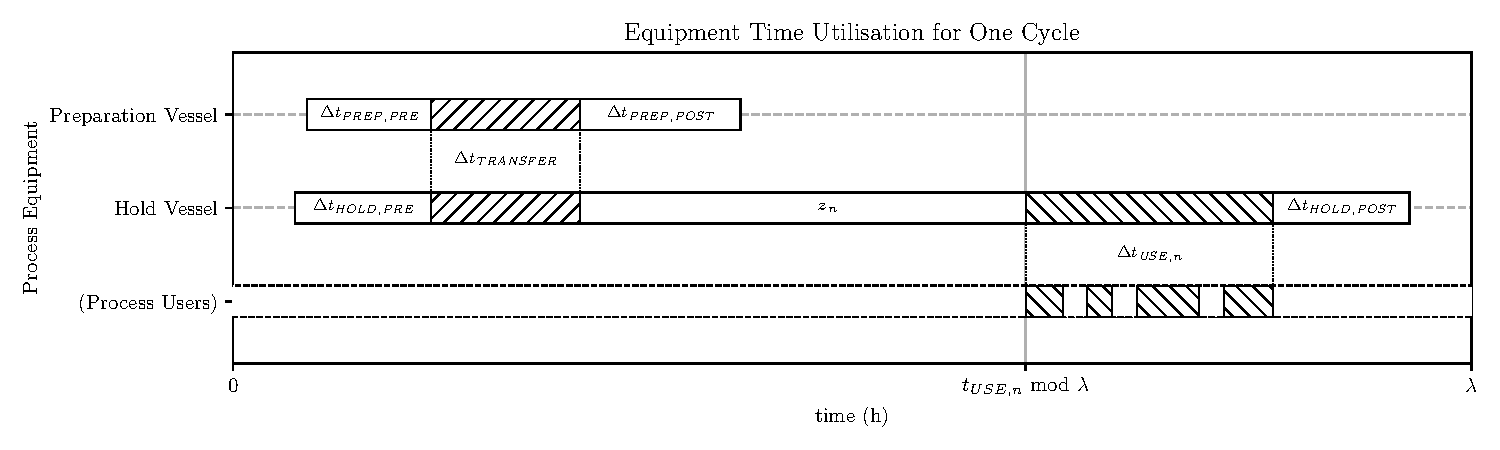
\includegraphics[width=0.99\textwidth]{./../figures/explanatory.pdf}
                    \caption{\Large \centering Schedule for a single buffer,
                        for a single batch.
                        Plot shows input timing parameters and the buffer hold
                        duration decision variable, $\boldsymbol{z}_n$.
                        Use of the buffer by the process may be discontinuous.}
                \end{figure}
            \column{0.33\textwidth}
                \begin{figure}
                    \includegraphics[width=0.85\textwidth]{timings.pdf}
                    \caption{\Large \centering Solution duration as a function
                        of problem size and solver selection -- each data point
                        is the arithmetic mean of 100 iterations.}
                \end{figure}
         \end{columns}
         \begin{columns}[t]
                \column{0.44\textwidth}
                \begin{block}{\huge Methodology}
                    The problem was modelled as a mixed-integer linear
                    programming (MILP) problem.
                    %\begin{itemize}                 
                    %    \item The objective function (to be minimised) is the
                    %        total cost of preparation vessels.\\
                    %    \item Each buffer must be prepared in a particular 
                    %        \emph{slot} (a notional space that may contain a
                    %        vessel).
                    %    \item Each slot may contain at most one vessel.
                    %    \item Each vessel must be adequately sized.
                    %    \item{Preparation vessels must not be over-utilised}
                    %             
                    %    \item Buffer hold procedure must be shorter than cycle
                    %        time.
                    %    \item Preparation procedures mustn't clash in time.
                    %    \item Constrain total vessel cost to be equal to the
                    %        objective function value from the complete problem.
                    %    \item Set the minimisation of buffer hold durations as
                    %        the new objective.
                    %\end{itemize}
                \end{block}
                \begin{block}{\huge Implementation}
                    \begin{itemize}
                        \item MILP model solved via the python PuLP API.
                        \item The CPLEX, Cbc and GLPK solvers were used.
                    \end{itemize}
                \end{block}
                \begin{block}{\huge Business Contribution}
                    \begin{itemize}
                        \item Reduces time taken to generate early-stage
                            designs.
                        \item Method developed provides provably optimum
                            solutions; previous methods did not.
                        \item Ability for a design firm to provide a provably
                            optimum solution, with supporting graphics,
                            increases the value of their design offering.
                    \end{itemize}
                \end{block}
                \begin{block}{\huge Academic Contribution}
                    Work in the field of bioprocessing design has, to date,
                    largely concentrated on the area of \emph{process design},
                    whereas this study looks at \emph{facility design},
                    contributing to the fields of biotechnology and
                    linear programming.
                \end{block}
                \begin{block}{\huge Scope for Further Work}
                    \begin{itemize}
                        \item Add more complexity/features to model.
                        \item Use model in conjunction with Monte Carlo
                            simulation to ensure designs can cope with
                            variability
                    \end{itemize}
                \end{block}
            \column{0.50\textwidth}
                \begin{block}{\huge Results}
                    For the data set shown above; one \SI{2000}{\litre} vessel,
                    one \SI{8000}{\litre} litre vessel, one \SI{25000}{\litre}
                    vessel and one \SI{30000}{\litre} litre vessel are
                    required for buffer preparation.
                    Results are best visualised in an \emph{equipment time
                    utilisation} plot.
                \end{block}
                \begin{figure}
                    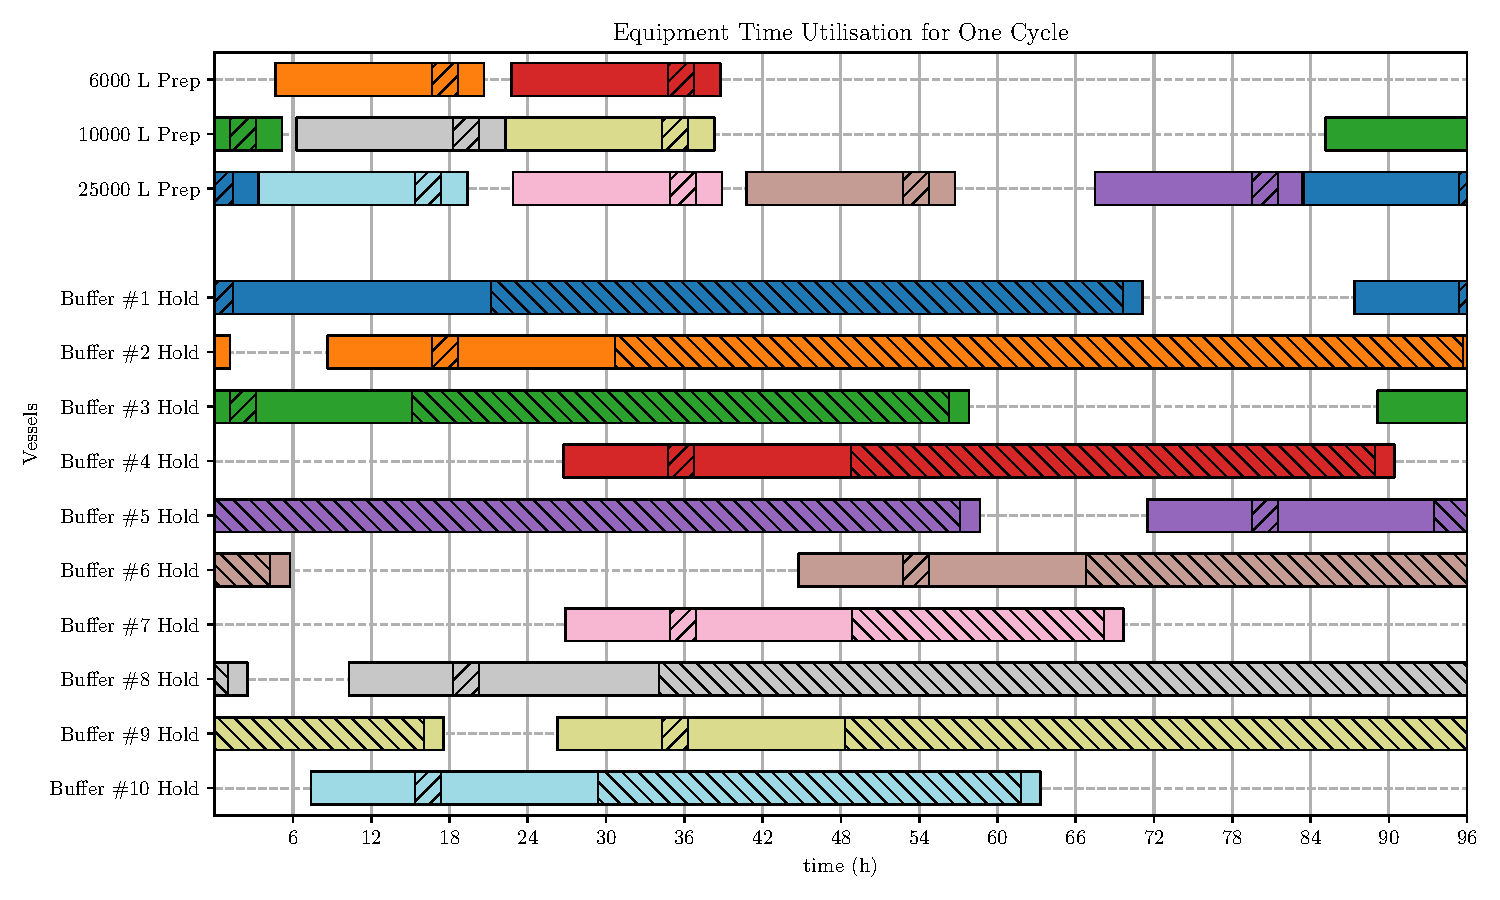
\includegraphics[width=0.993\textwidth]{./../figures/plot2.pdf}
                    \captionsetup{justification=centering}
                    \caption{\Large Equipment Time Utilisation
                    plot showing a feasible schedule for a single cycle window
                    at steady-state with minimal buffer vessel cost.}
                \end{figure}
                \begin{block}{\huge Conclusions}
                    \begin{itemize}
                        \item A working, usable model was developed which
                            generated optimal results.
                        \item Solution time is exponential in the number of
                            buffers.
                    \end{itemize}
                \end{block}
        \end{columns}
    
    \vspace{0.3cm}
    
    \large\centering Check out the source code at:
    \url{https://github.com/multipitch/dissertation}
    \end{frame}
\end{document}
